% --- IMPORTS ---
\documentclass[leqno]{article}
\usepackage{graphicx}
\usepackage{dsfont}
\usepackage{mathtools}
\usepackage{amssymb}
\usepackage{amsmath}
\usepackage{amsthm}
\usepackage{float}
\usepackage{ragged2e}
\usepackage{tensor}
\usepackage{fancyhdr}
\usepackage{empheq}
\usepackage[most]{tcolorbox}
\usepackage{enumitem}
\usepackage{dirtytalk}
\usepackage{marginnote}
\usepackage{microtype}
\usepackage[
  a4paper,
  left=0.8in,
  right=1in,
  top=1in,
  bottom=0.5in,
  headheight=14pt,
  headsep=0.4in
]{geometry}
\setlength{\parindent}{0cm}
% --- TikZ Packages ---
\usepackage{pgfplots}
\pgfplotsset{compat=1.18}
\usepgfplotslibrary{fillbetween, polar}
\usetikzlibrary{calc, positioning}
\usetikzlibrary{angles, quotes}
\usetikzlibrary{arrows.meta}
\usetikzlibrary{decorations.pathreplacing, decorations.markings}
\usetikzlibrary{patterns}
\usetikzlibrary{intersections}
% --- URL Packages ---
\usepackage[colorlinks=true,linkcolor=red,citecolor=magenta,urlcolor=black]{hyperref}%
\urlstyle{same}
% --- END OF IMPORTS ---

% --- CUSTOM COMMANDS ---
\RenewDocumentCommand{\marks}{o m}{%
  \IfValueTF{#1}%
    {\marginnote{\raggedright\textbf{[#2]}}[#1]}%
    {\marginnote{\raggedright\textbf{[#2]}}}%
}
\newcommand{\vspacerule}[2]{%
  \par\vspace*{#1}%
  \noindent\hrulefill\par
  \vspace*{#2}%
}
\definecolor{scarlet}{RGB}{205, 40, 75}
\newcommand{\questionitem}{%
  \item\phantomsection
  \addcontentsline{toc}{section}{Question \number\value{enumi}}%
}
\renewcommand{\contentsname}{Questions}
% --- END OF CUSTOM COMMANDS ---

% --- HEADER CONFIG ---
\pagestyle{fancy}
\fancyhead{}
\fancyfoot{}
\renewcommand{\headrulewidth}{0.9pt}
\lhead{Integration by Parts (FM Level)}
\chead{}
\rhead{\href{https://danieljsmith.org}{danieljsmith.org}}
% --- END OF HEADER CONFIG ---

\begin{document}
\vspace*{20pt}
\tableofcontents
\newpage
\begin{enumerate}[
  label=\textbf{\arabic*.},
  leftmargin=*,
  topsep=0pt,
  partopsep=0pt,
  parsep=0pt
]

% ---- Question 1 ----
\questionitem

Given that
\[
y = \arctan\left(\frac{x-2}{x+2}\right)
\]
where $x\ne -2$ \\
\begin{enumerate}[label=\textbf{(\alph*)}]
  \item find $\dfrac{\mathrm{d}y}{\mathrm{d}x}$, giving your answer in its simplest form. \marks{2} \\
  \item Use integration by parts to find
  \[
  \int \arctan\left(\frac{x-2}{x+2}\right)\,\mathrm{d}x
  \]
  \marks[-20pt]{4}
\end{enumerate}
\newpage
% ---- Question 2 ----
\questionitem
Use integration by parts to find


  \[
  \int_0^2 x^2 \ln(1+x)\,\mathrm{d}x
  \]
  
  giving your answer in the form $a + b\ln 3$, where $a$ and $b$ are constants to be found. \marks{5} \\
  

\newpage
% ---- Question 3 ----
\questionitem

Use integration by parts to find 

\[
\int \operatorname{arsinh}(2x+1)\, \mathrm{d}x
\]

giving your answer in terms of logarithms. \marks{5}

\newpage

% ---- Question 4 ----
\questionitem

\[
h(\theta)=(3\sin\theta-\cos\theta)(\sin\theta+2\cos\theta)
\] \\
\begin{enumerate}[label=\textbf{(\alph*)}]
  \item Show that $h(\theta)=\dfrac{1}{2}-\dfrac{5}{2}\cos 2\theta+\dfrac{5}{2}\sin 2\theta$. \marks{4} \\
  \item Hence, using calculus, find the exact value of
  \[
  \int_{0}^{\frac{\pi}{2}} \left(\frac{\pi}{2}-\theta\right) h(\theta)\,\mathrm{d}\theta
  \]
  \marks[-30pt]{7}
\end{enumerate}

\newpage

% ---- Question 5 ----
\questionitem

\begin{enumerate}[label=\textbf{(\alph*)}]
  \item Find
  \[
  \int x^2\arctan x\,\mathrm{d}x
  \]
  \marks[-20pt]{5}
  \item Hence find the exact value of
  \[
  \int_0^1 x^2\arctan x\,\mathrm{d}x
  \]
  \marks[-20pt]{2}
\end{enumerate}

\newpage

% ---- Question 6 ----
\questionitem

\begin{enumerate}[label=\textbf{(\roman*)}]
  \item Sketch the graph of $y=\arctan x$ for $x\in\mathbb{R}$, indicating any horizontal asymptotes. \marks{1} \\
  \item Prove that
  \[
  \frac{\mathrm{d}}{\mathrm{d}x}(\arctan x)=\frac{1}{1+x^2}
  \]
  \marks[-20pt]{4}
  \item Using integration by parts and suitable substitutions, show that
  \[
  \int_0^1 x(\arctan x)^2\,\mathrm{d}x=\frac{\pi^2}{16}-\frac{\pi}{4}+\frac{1}{2}\ln 2
  \]
  \marks[-30pt]{6}
\end{enumerate}

\newpage

% ---- Question 7 ----
\questionitem

\begin{enumerate}[label=\textbf{(\alph*)}]
  \item Find
  \[
  \int x^3\arctan x\,\mathrm{d}x
  \]
  \marks[-20pt]{5}
  \item Hence find the exact value of
  \[
  \int_0^{\sqrt{3}} x^3\arctan x\,\mathrm{d}x
  \]
  \marks[-20pt]{2}
\end{enumerate}

\newpage

% ---- Question 8 ----
\questionitem

\begin{enumerate}[label=\textbf{(\alph*)}]
  \item Using the logarithmic form
  \[
  \operatorname{artanh} x = \frac{1}{2}\ln\left(\frac{1+x}{1-x}\right),\qquad |x|<1
  \]
  prove that the derivative of $\operatorname{artanh} x$ is
  \[
  \frac{1}{1-x^2}
  \]
  \marks{5} \\
  \item Hence find
  \[
  \int_0^{1/3} \operatorname{artanh}(2x)\,\mathrm{d}x
  \]
  giving your answer in exact logarithmic form. \marks{5} \\
  \item Noah tries to evaluate
  \[
  \int_0^{1/2} \operatorname{artanh}(2x)\,\mathrm{d}x
  \]
  using his calculator, and gets an error. Explain why. \marks{1} \\
\end{enumerate}

\newpage

% ---- Question 9 ----
\questionitem

For $0<x<1$, use integration by parts to find
\[
\int x\,\operatorname{artanh}(2x-1)\,\mathrm{d}x
\]
giving your final answer in terms of logarithms. \marks{6}

\newpage

% ---- Question 10 ----
\questionitem

\begin{figure}[H]
    \centering
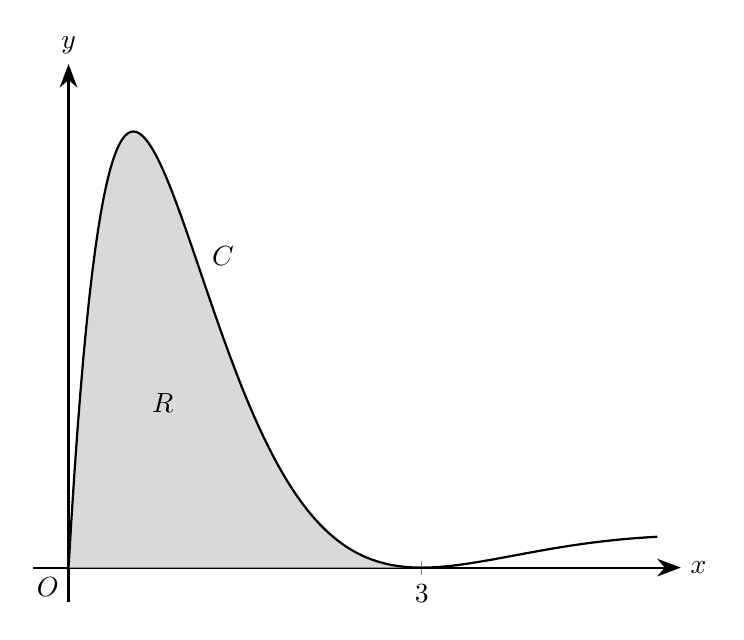
\begin{tikzpicture}[scale=1.2]
\begin{axis}[
    axis lines=middle,
    axis line style={-{Stealth[length=3mm]}, thick},
    xlabel={$x$},
    ylabel={$y$},
    xmin=-0.3, xmax=5.2,
    ymin=-0.15, ymax=2.2,
    xtick={3},
    xticklabels={$3$},
    ytick=\empty,
    clip=false,
    every axis x label/.style={at={(ticklabel* cs:1)}, anchor=west},
    every axis y label/.style={at={(ticklabel* cs:1)}, anchor=south}
]
\addplot[draw=none, name path=curvefill, samples=200, domain=0:5.0] {x*(3 - x)^2*exp(-x)};
\addplot[draw=none, name path=axisfill, domain=0:5.0] {0};
\addplot[gray!30] fill between[of=curvefill and axisfill, soft clip={domain=0:3}];
\addplot[thick, black, samples=200, domain=0:5.0] {x*(3 - x)^2*exp(-x)} node[pos=0.4, above right] {$C$};
\node at (axis cs:0.8,0.72) {$R$};
\node[below left] at (axis cs:0,0) {$O$};
\end{axis}
\end{tikzpicture}
\end{figure}


The sketch shows part of the curve $C$ given by\\

\[
y = x(3-x)^2 e^{-x} \qquad x \geq 0
\] \\
The shaded region $R$ is bounded by $C$ and the $x$-axis for $0 \leq x \leq 3$. \\

Find the exact area of $R$, giving your answer in the form
\[
A + Be^{-3}
\]
where $A$ and $B$ are rational numbers. \marks{5}

\newpage

% ---- Question 11 ----
\questionitem

Show that\\

\[
\int_{e^{-1/2}}^1 x(\ln x)^2\,\mathrm{d}x = a + \frac{b}{e}
\]\\

where $a$ and $b$ are rational constants to be found. \marks{6}

\newpage


% ---- Question 12 ----
\questionitem

\begin{enumerate}[label=\textbf{(\alph*)}]
  \item Using the logarithmic form of $\operatorname{artanh} x$, prove that the derivative of $\operatorname{artanh} x$ is
  \[
  \frac{1}{1-x^2}
  \]
  for $|x|<1$. \marks{5} \\
  \item Hence find
  \[
  \int_0^{1/2} \operatorname{artanh} x\,\mathrm{d}x
  \]
  giving your answer in exact logarithmic form. \marks{5} \\
  \item Priya tries to evaluate
  \[
  \int_0^{3/2} \operatorname{artanh} x\,\mathrm{d}x
  \]
  using her calculator, and gets an `error'. Explain why. \marks{1} \\
\end{enumerate}

\newpage


% ---- Question 13 ----
\questionitem

Given that
\[
y = \arcsin\left(\frac{x-1}{3}\right)
\] \\
\begin{enumerate}[label=\textbf{(\alph*)}]
  \item find $\dfrac{\mathrm{d}y}{\mathrm{d}x}$, giving your answer in its simplest form. \marks{2} \\
  \item Use integration by parts to find
  \[
  \int \arcsin\left(\frac{x-1}{3}\right)\,\mathrm{d}x
  \]
  \marks[-20pt]{4}
\end{enumerate}

\newpage

% ---- Question 14 ----
\questionitem

Use integration by parts to find
\[
\int_1^9 \sqrt{x}\ln\left(\frac{9}{x}\right)\,\mathrm{d}x
\]
giving your answer in the form $a + b\ln 3$, where $a$ and $b$ are constants to be found. \marks{5}

\newpage

% ---- Question 15 ----
\questionitem

\[
g(\theta)=(1+\sin\theta-\cos\theta)^2
\] \\
\begin{enumerate}[label=\textbf{(\alph*)}]
  \item Show that $g(\theta)=2+2\sin\theta-2\cos\theta-\sin 2\theta$. \marks{4} \\
  \item Hence, using calculus, find the exact value of
  \[
  \int_{0}^{\frac{\pi}{2}} \theta g(\theta)\,\mathrm{d}\theta
  \]
  \marks[-30pt]{7}
\end{enumerate}
\end{enumerate}
\end{document}
